\documentclass[11pt,letterpaper]{report}
\usepackage[latin1]{inputenc}
\usepackage{amsmath}
\usepackage{amsfonts}
\usepackage{amssymb}
\usepackage{graphicx}
\usepackage{color}
\usepackage{enumitem}
\usepackage[dvipsnames]{xcolor}
\definecolor{codegray}{gray}{0.9}
\newcommand{\code}[1]{\colorbox{codegray}{\texttt{#1}}}
\graphicspath{{./images/}{IR}}
%\newcommand{\LF}{}  % turn on to display large format
\ifdefined \LF
\usepackage[left=2.0cm, top=2.0cm, landscape]{geometry}  % for large format landscape
\else
\usepackage[left=2.0cm, top=2.0cm]{geometry}
\fi
\usepackage{fancyhdr}
\pagestyle{fancy}
\fancyhead{}
\lhead{CS333}
\chead{Project 3 Test Report}
\rhead{Alexander DuPree}
\begin{document}
\title{Project 3 Test Report}
\author{Alexander DuPree}

\ifdefined \LF
{\Large     % large print start
\fi

  \maketitle
  \section*{Introduction}
  \noindent
  The following test report documents the tests performed for project three. The test cases and strategies closely follow the project three rubric. 

  Each section contains test cases related to the sections topic. Each test case will describe the name of the test, 
  the expected result, actual result, as well as a discussion and indication of the Pass/Fail status. 
  The actual result will be provided in the form of a screen shot of the console. 

  \section*{Compilation}
  This section presents all tests related to compiling the xv6 kernel.
  Test cases follow closely those outlined in the rubric. \hfill \break
  
  \noindent\textbf{Test Case:} \emph{With CS333\_PROJECT set to 0 in the Makefile}
  
  \noindent\textbf{Assertions:}
  \begin{enumerate}[]
  \item Code correctly compiles
  \item Kernel successfully boots
  \item \code{usertests} run to completion with all tests passed
  \end{enumerate}  
  
  \noindent\textbf{Status:} \textcolor{ForestGreen}{\textbf{PASS}}
  
  \begin{figure}[h!]
	\centering
	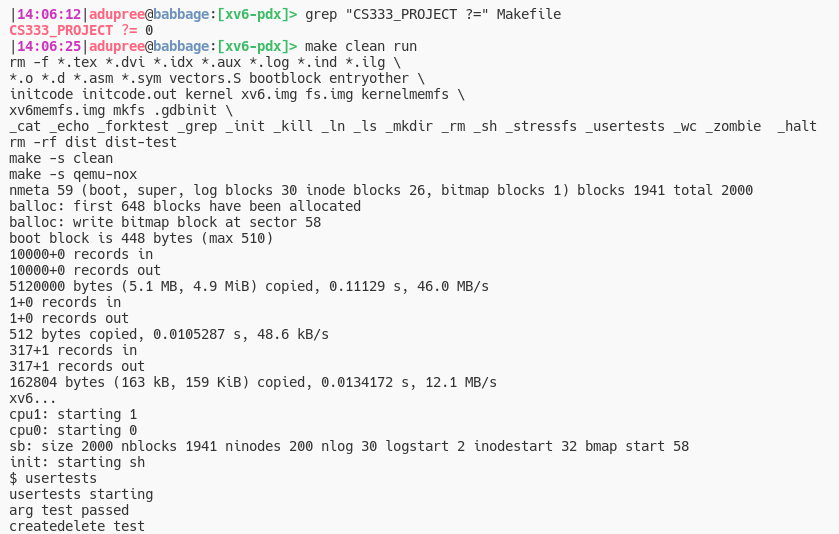
\includegraphics[width=1\linewidth]{compilation1-usertests1.png}
	\caption[img]{Compilation and boot with CS333\_PROJECT set to 0 and execution of \code{usertests}}
	\label{fig:P1compileP0-1}
  \end{figure}

  \begin{figure}[h!]
	\centering
	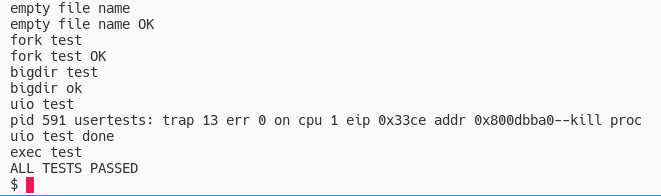
\includegraphics[width=1\linewidth]{compilation1-usertests2.png}
	\caption[img]{Completion of \code{usertests} with output elided}
	\label{fig:P1compileP0-1}
  \end{figure}

  The command \code{grep "CS333\_PROJECT ?=" Makefile} shows that the CS333\_PROJECT macro is set to 0.
  The following command \code{make clean run} demonstrates that the code correctly compiles and the kernel successfully boots. 
  Furthermore, the commands were executed within seconds of each other, indicating that
  tampering is not a possibility. Lastly, we can see that the execution of \code{usertests}
  is initiated in the same session, and Figure 2 shows that the tests run to completion and 
  all tests pass. \\

  \noindent\textbf{Test Case:} \emph{With CS333\_PROJECT set to 3 in the Makefile}
  
  \noindent\textbf{Assertions:}
  \begin{enumerate}[]
  \item Code correctly compiles
  \item Kernel successfully boots
  \item \code{usertests} run to completion with all tests passed
  \end{enumerate}  
  
  \noindent\textbf{Status:} \textcolor{ForestGreen}{\textbf{PASS}}
  
  \begin{figure}[h!]
	\centering
	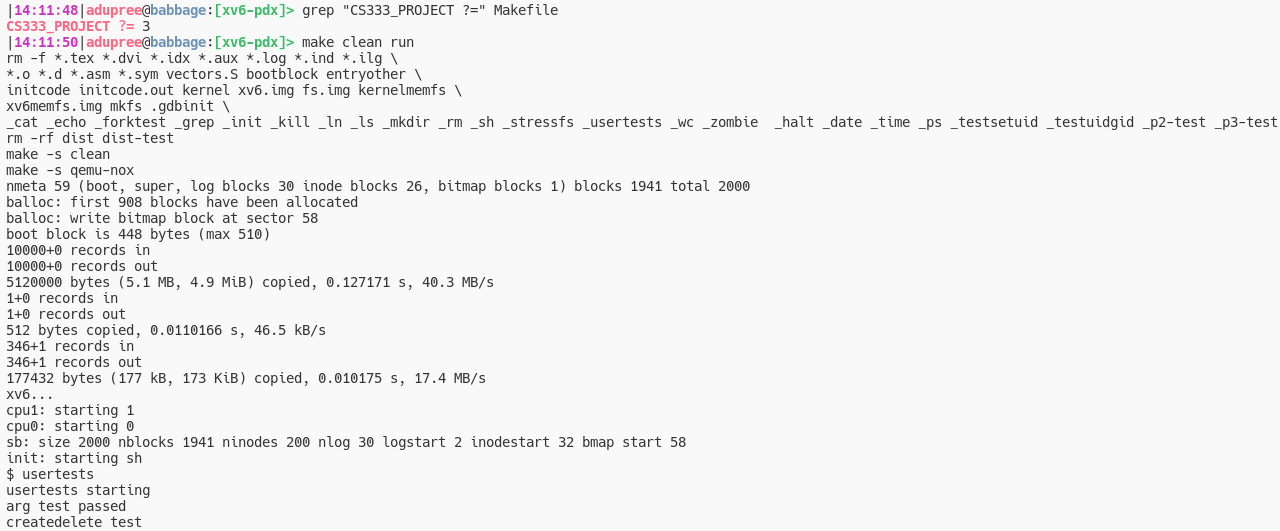
\includegraphics[width=1\linewidth]{compilation2-usertests1.png}
	\caption[img]{Compilation and boot with CS333\_PROJECT set to 3 and execution of \code{usertests}.}
	\label{fig:P1compileP0-1}
  \end{figure}

  \begin{figure}[h!]
	\centering
	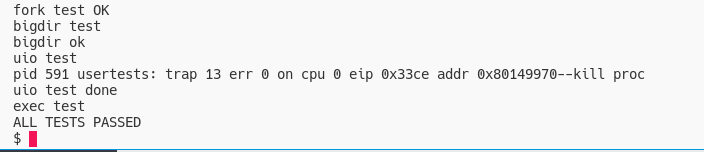
\includegraphics[width=1\linewidth]{compilation2-usertests2.png}
	\caption[img]{Completion of \code{usertests} with output elided, CS333\_P3 is defined}
	\label{fig:P1compileP0-1}
  \end{figure}

  The command \code{grep "CS333\_PROJECT ?=" Makefile} shows that the CS333\_PROJECT macro
  is indeed set to 3. The following command \code{make clean run} demonstrates that the code
  correctly compiles and the kernel successfully boots. Furthermore, the commands were executed
  within seconds of each other, indicating that tampering is not a possibility. Lastly, we can
  see that the execution of \code{usertests} is initiated in the same session and Figure 4
  demonstrates that the tests run to completion and all tests pass. \\

  \pagebreak

  \section*{State Lists and Console Commands}
  This section presents all tests related to the initilization, use, and maintenance
  of the kernels process state lists and debug console commands. 
  Test cases follow closely those outlined in the rubric. \hfill \break
  
  \noindent\textbf{Test Case:} \emph{Initialization and use of \code{UNUSED} list and CTRL+F console interrupt}
  
  \noindent\textbf{Assertions:}
  \begin{enumerate}[]
  \item \code{UNUSED} list is correctly initialized after Xv6 boots
  \item \code{UNUSED} list is correctly updated when a process is allocated and deallocated
  \item CTRL+F correctly shows the number of \code{UNUSED} processes.
  \end{enumerate}  
  
  \noindent\textbf{Status:} \textcolor{ForestGreen}{\textbf{PASS}}
  
  \begin{figure}[h!]
	\centering
	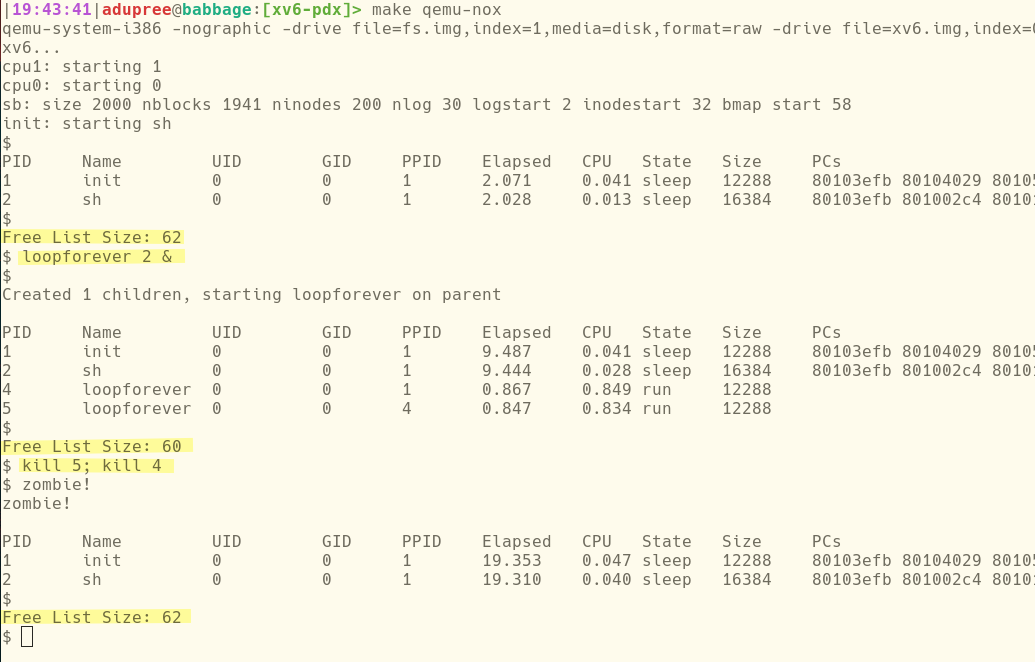
\includegraphics[width=1\linewidth]{unused-list1.png}
	\caption[img]{Checking free list size after boot, creating two procsses, re-checking list size, killing the two processes, final list size check}
	\label{fig:P1compileP0-1}
  \end{figure}

  After Xv6 boots we immediately use CTRL+P to display init and sh processes, then we 
  use CTRL+F to print out the number of processes in the \code{UNUSED} list. Since the 
  max number of procs is 64, and there are 2 used processes after startup, we can conclude
  that 62 is the correct number of processes in the \code{UNUSED} list. This proves our
  first assertion that the \code{UNUSED} list is correclty initialized after boot to be true. 
  
  Next, we create 2 new background processes with \code{loopforever 2 \&}. 
  The program \code{loopforever} is a simple user program that, when given an integer N, will
  create N-1 children processes that will loop forever, after which the parent itself will also 
  loop forever. After creating the processes we use the same sequence of CTRL+P to display 
  all used processes and CTRL+F to get the current length of the \code{UNUSED} list. Since, 
  after creating 2 more processes, the length of the \code{UNUSED} list is 60 we can conclude
  that the \code{UNUSED} list is correctly updated after process allocation.

  Lastly, we kill the newly created processes and then use CTRL+P and CTRL+F to get the 
  state of the operation system. The bottom of Figure 5 shows that after killing the 
  processes the size of the free list is once again 62. This demonstrates that the 
  \code{UNUSED} list is being correctly updated after a process is deallocated. \\

  \pagebreak

  \noindent\textbf{Test Case:} \emph{\code{RUNNABLE} list, round-robin scheduling, and CTRL+R console interrupt}
  
  \noindent\textbf{Assertions:}
  \begin{enumerate}[]
  \item \code{RUNNABLE} list is correctly updated to contain all \code{RUNNABLE} processes
  \item Round-Robin scheduling is maintained
  \item CTRL+R correctly shows the current order of the \code{RUNNABLE} list.
  \end{enumerate}  
  
  \noindent\textbf{Status:} \textcolor{ForestGreen}{\textbf{PASS}}
  
  \begin{figure}[h!]
	\centering
	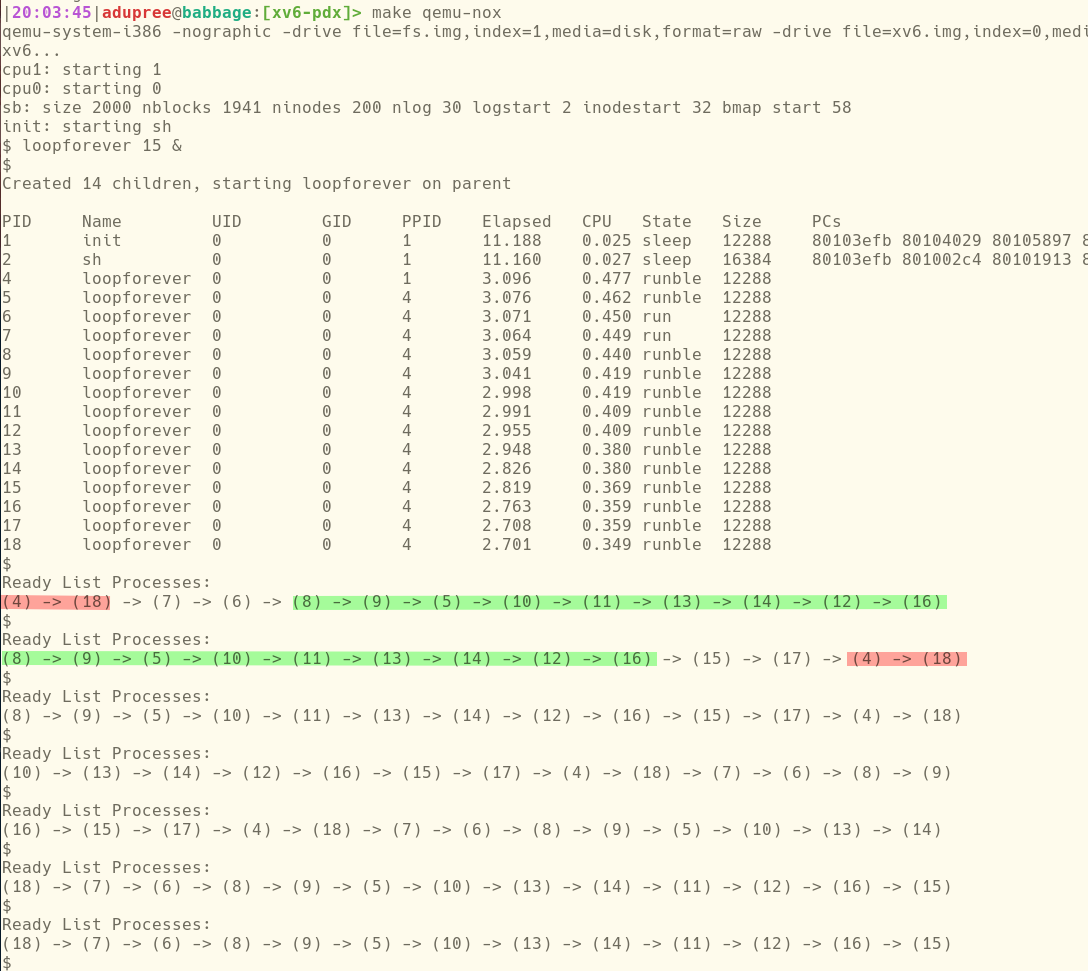
\includegraphics[width=1\linewidth]{round-robin.png}
	\caption[img]{Creating 15 background processes and holding down CTRL+R}
	\label{fig:P1compileP0-1}
  \end{figure}

  For this test we use the command \code{loopforever 15 \&} to instantiate 15 background
  processes that will increment a counter variable in an infinite loop. After we create 
  processes we use CTRL+P to show that all our processes are either in the \code{RUNNABLE} 
  or \code{RUNNING} states. After which, we hold down CTRL+R to display the current order 
  of the \code{RUNNABLE} list. At first, the red highlighted processes are at the head of the 
  list. Then, after the interrupt regisers again we can see the same sequence of processes
  is now at the back of the list and the green highlighted processes have moved toward 
  the front of the list. This demonstrates that the round-robin scheduling is being 
  maintained.\\

  \noindent\textbf{Test Case:} \emph{\code{SLEEPING} list and CTRL+S console interrupt}
  
  \noindent\textbf{Assertions:}
  \begin{enumerate}[]
  \item \code{SLEEPING} list is correctly updated when a process sleeps and is woken up.
  \item CTRL+S correctly displays all \code{SLEEPING} processes
  \end{enumerate}  
  
  \noindent\textbf{Status:} \textcolor{ForestGreen}{\textbf{PASS}}
  
  \begin{figure}[h!]
	\centering
	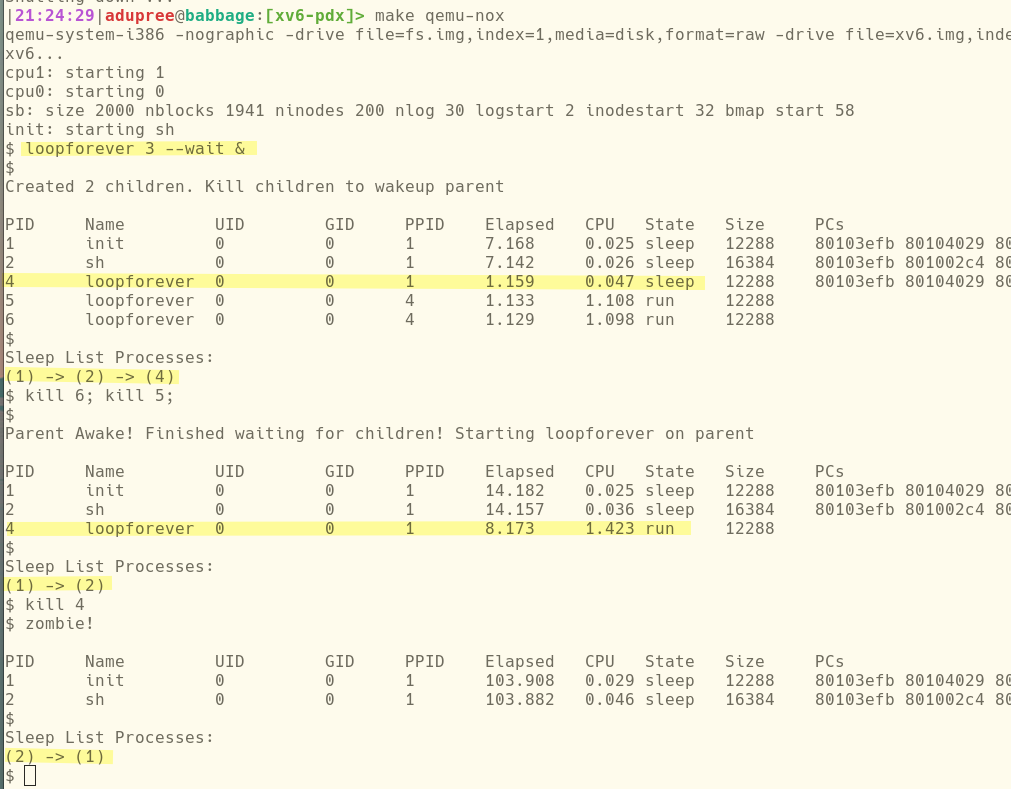
\includegraphics[width=1\linewidth]{sleeptest.png}
	\caption[img]{Running loopforever with parent asleep, and resulting sleep list after child exits}
	\label{fig:P1compileP0-1}
  \end{figure}

  To demonstrate that the \code{SLEEPING} list is being properly maintained we first run
  the command \code{loopforever 3 --wait \&}. The \code{--wait} flag will tell the 
  parent process to wait (and thus go to sleep) for its 2 children. We can see that 
  after using CTRL+P and CTRL+S that the parent process, with a PID of 4, is indeed asleep, and is at 
  the back of the sleep list. After killing the parents children the parent will be woken 
  up and then start its infinite loop. We can see this in Figure 7, the parent process is 
  in the 'run' state and is no longer on the sleep list processes. Furthermore, when we kill
  the parent process the \code{init} process will be awoken to deal with the Zombie and then
  placed back onto the \code{SLEEPING} list. This is proven to be true at the bottom of 
  Figure 7, since we can see that the init process (PID 1) is now at the back of the list. 
  Lastly, this is also further evidence that the wait system call moves the reaped children
  back to the \code{UNUSED} list, since the child processes appear in CTRL+P interrupt.

\ifdefined \LF
} % large print end
\fi

\end{document}